% -*- LaTeX -*-
% -*- coding: utf-8 -*-
%
% michael a.g. aïvázis
% california institute of technology
% (c) 1998-2012 all rights reserved
%

\lecture{The distributed memory implementation}{20120229}

% --------------------------------------
% parallelization with MPI
\begin{frame}[fragile]
%
  \frametitle{Parallelization with \mpi}
%
  \begin{itemize}
%
  \item the \mpi\ implementation will require careful data management
    \begin{itemize}
    \item we must partition the mesh among processes
    \item each process work on its own subgrid
      \begin{itemize}
      \item it will allocate its own memory, for both actual data and the guard zones
      \item it must locate its patch in physical space
      \end{itemize}
    \item communication is required every iteration
      \begin{itemize}
      \item so that neighbors can synchronize their boundaries
      \item think of the synchronization as a kind of boundary condition!
      \end{itemize}
    \item parallel convergence testing involves a collective operation
    \end{itemize}
%
  \end{itemize}
%
  \begin{figure}
    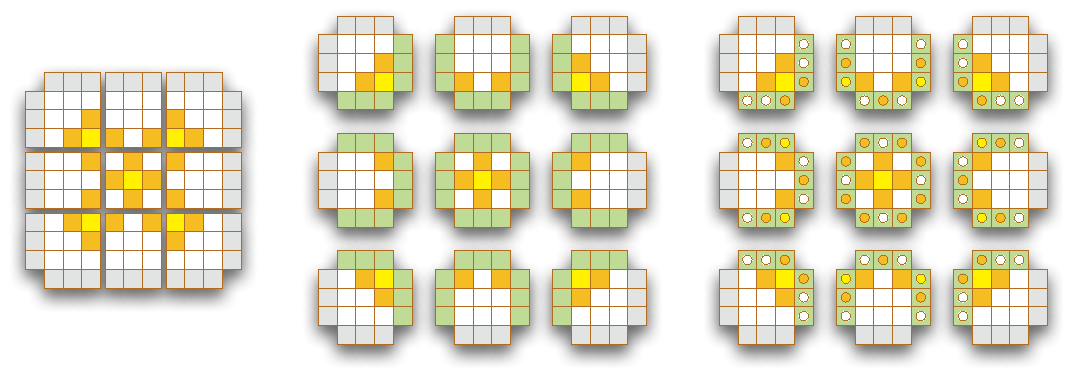
\includegraphics[scale=0.5]{figures/structured-partitioning.pdf}
  \end{figure} 
% 
\end{frame}

% --------------------------------------
% template
\begin{frame}[fragile]
%
  \frametitle{A little bit of help}
%
  \begin{itemize}
%
  \item \mpi\ supports this common use case through a Cartesian {\em virtual topology}
    \begin{itemize}
    \item a special communicator with a map from a $d$-dimensional virtual process grid to the
      normal linear process ranks
    \item and local operations that enable you to discover the ranks of your virtual neighbors
    \item there is even a special form of send/receive so that you don't have to worry about
      contention and race conditions during the boundary synchronization
    \end{itemize}
%
  \item to create a Cartesian communicator
    \begin{C}
int MPI_Cart_create(MPI_Comm oldcomm,
        int ndims, int* layout, int* periods, int reorder, MPI_Comm* newcomm);
    \end{C}
%
  \item to find out the coordinates of a process in the virtual grid given its rank
    \begin{C}
int MPI_Cart_coords(MPI_Comm cartesian,
        int rank, int ndims, int* coords); 
    \end{C}
%
    \item you can also find out the ranks of your neighbors
    \begin{C}
int MPI_Cart_shift(MPI_Comm cartesian,
        int dimension, int shift, int* origin, int* neighbor); 
    \end{C}
%
  \end{itemize}
%
\end{frame}

% --------------------------------------
% the mpi driver
\begin{frame}[fragile]
%
  \frametitle{The \mpi\ driver, part 1}
%
  \begin{lstlisting}[language=c++,name=mpi:driver,firstnumber=26,basicstyle=\tt\bfseries\tiny]
int main(int argc, char* argv[]) {
    int status;
    // initialize mpi
    status = MPI_Init(&argc, &argv);
    if (status) {
        throw("error in MPI_Init");
    }
    // get my rank in the world communicator
    int worldRank, worldSize;
    MPI_Comm_rank(MPI_COMM_WORLD, &worldRank);
    MPI_Comm_size(MPI_COMM_WORLD, &worldSize);
    size_t processors = static_cast<size_t>(std::sqrt(worldSize));

    // default values for our user configurable settings
    size_t n = 9; // points per processor
    size_t threads = 1;
    double tolerance = 1.0e-3;

    // read the command line
    int command;
    while ((command = getopt(argc, argv, "n:e:t:")) != -1) {
        switch (command) {
        // get the convergence tolerance
        case 'e':
            tolerance = atof(optarg);
            break;
        // get the grid size
        case 'n':
            n = (size_t) atof(optarg);
            break;
        // get the number of threads
        case 't':
            threads = (size_t) atoi(optarg);
            break;
        }
    }
  \end{lstlisting}
% 
\end{frame}

% --------------------------------------
% the mpi driver
\begin{frame}[fragile]
%
  \frametitle{The \mpi\ driver, part 2}
%
  \begin{lstlisting}[language=c++,name=mpi:driver,basicstyle=\tt\bfseries\tiny]
    // print out the chosen options
    if (worldRank == 0) {
        for (int arg = 0; arg < argc; ++arg) {
            std::cout << argv[arg] << " ";
        }
        std::cout
            << std::endl
            << "    grid size: " << n << std::endl
            << "      workers: " << threads << std::endl
            << "    tolerance: " << tolerance << std::endl;
    }

    // instantiate a problem
    Example problem("cliche", 1.0, processors, n);

    // instantiate a solver
    Jacobi solver(tolerance, threads);
    // solve
    solver.solve(problem);
    // save the results
    Visualizer vis;
    vis.csv(problem);

    // initialize mpi
    status = MPI_Finalize();
    if (status) {
        throw("error in MPI_Finalize");
    }

    // all done
    return 0;
}
  \end{lstlisting}
% 
\end{frame}

% --------------------------------------
% the mpi driver
\begin{frame}[fragile]
%
  \frametitle{The \class{Jacobi} declaration}
%
  \begin{lstlisting}[language=c++,name=mpi:jacobi-decl,basicstyle=\tt\bfseries\tiny]
class acm114::laplace::Jacobi : public acm114::laplace::Solver {
    // interface
public:
    virtual void solve(Problem &);

    // meta methods
public:
    inline Jacobi(double tolerance, size_t workers);
    virtual ~Jacobi();

    // data members
private:
    double _tolerance;
    size_t _workers;

    // disable these
private:
    Jacobi(const Jacobi &);
    const Jacobi & operator= (const Jacobi &);
};
  \end{lstlisting}
% 
\end{frame}

% --------------------------------------
% the problem base class
\begin{frame}[fragile]
%
  \frametitle{The \class{Problem} declaration}
%
  \begin{lstlisting}[language=c++,name=mpi:problem-decl,basicstyle=\tt\bfseries\tiny]
class acm114::laplace::Problem {
    //typedefs
public:
    typedef std::string string_t;
    // interface
public:
    string_t name() const;
    inline MPI_Comm communicator() const;
    inline int rank() const;
    // access to my grid
    inline Grid & solution();
    inline const Grid & solution() const;
    // interface used by the solver
    virtual void initialize();
    virtual void applyBoundaryConditions() = 0;
    // meta methods
public:
    Problem(string_t name, double interval, int processors, size_t points);
    virtual ~Problem();
    // data members
protected:
    string_t _name;
    double _delta, _x0, _y0;
    int _rank, _size, _processors;
    int _place[2];
    MPI_Comm _cartesian;
    Grid _solution;
    // disable these
private:
    Problem(const Problem &);
    const Problem & operator= (const Problem &);
};
  \end{lstlisting}
% 
\end{frame}

% --------------------------------------
% problem definitions
\begin{frame}[fragile]
%
  \frametitle{The \class{Problem} constructor}
%
  \begin{lstlisting}[language=c++,name=mpi:driver,basicstyle=\tt\bfseries\tiny]
Problem::Problem(
    string_t name, double interval, int processors, size_t points) :
    _name(name),
    _delta(interval/((points-2)*processors+1)),
    _x0(0.0), _y0(0.0),
    _rank(0), _size(0), _processors(processors), _place(),
    _cartesian(),
    _solution(points) {

    // build the intended layout
    int layout[] = { processors, processors };
    // find my rank in the world communicator
    int worldRank;
    MPI_Comm_rank(MPI_COMM_WORLD, &worldRank);
    // build a Cartesian communicator
    int periods[] = { 0, 0 };
    MPI_Cart_create(MPI_COMM_WORLD, 2, &layout[0], periods, 1, &_cartesian);
    // check whether i can paritcipate
    if (_cartesian != MPI_COMM_NULL) {
        // get my rank in the cartesian communicator
        MPI_Comm_rank(_cartesian, &_rank);
        MPI_Comm_size(_cartesian, &_size);
        // get my logical position on the process grid
        MPI_Cart_coords(_cartesian, _rank, 2, &_place[0]);
        // now compute my offset in physical space
        _x0 = 0.0 + (points-2)*_place[0]*_delta;
        _y0 = 0.0 + (points-2)*_place[1]*_delta;
    } else {
        // i was left out because the total number of processors is not a square
        std::cout
            << "world rank " << worldRank << ": not a member of the cartesian communicator "
            << std::endl;
    }
}
  \end{lstlisting}
% 
\end{frame}


% --------------------------------------
% the Example declaration
\begin{frame}[fragile]
%
  \frametitle{The \class{Example} declaration}
%
  \begin{lstlisting}[language=c++,name=mpi:example-decl]
class acm114::laplace::Example : public acm114::laplace::Problem {
    // interface
public:
    virtual void applyBoundaryConditions();

    // meta methods
public:
    inline Example(
        string_t name, double interval, int processors, size_t points);
    virtual ~Example();

    // disable these
private:
    Example(const Example &);
    const Example & operator= (const Example &);
};
  \end{lstlisting}
% 
\end{frame}

% end of file 
